\section{Nền tảng lý thuyết}

\subsection{Sơ lược về Bitcoin}
Các hình thức thương mại trên Internet ngày nay hầu như đều dựa vào một tổ chức 
bên thứ ba đáng tin cậy để xử lý các hoạt động thanh toán điện tử. Tuy rằng sau 
nhiều năm phát triển, các tổ chức bên thứ ba này đều đã nâng cao mức độ tin cậy, 
an toàn nhưng đa số vẫn còn tồn tại những điểm yếu: không thể tránh khỏi những 
tranh chấp, phí trung gian, đòi hòi phải cung cấp các thông tin cá nhân... Và 
Bitcoin - hệ thống tiền điện tử ngang hàng (A Peer-to-Peer Electronic Cash System) 
được sinh ra để giải quyết các vấn đề trên \cite{BitcoinPaper}.\\\\
Khi so sánh với tiền tệ truyền thống, Bitcoin có hình thức và cách thức hoạt 
động khác biệt. Bitcoin không hề có bất kỳ một tổ chức tập trung nào để quản 
lý, thay vào đó, Bitcoin sử dụng mạng ngang hàng để hoạt động \cite{Bitcoin1}.
\\\\
Trong cách viết, Bitcoin được hiểu như một hệ thống, giao thức hoặc một cộng 
đồng, cụ thể trong phạm vi bài dự thi này, Bitcoin được hiểu là một hệ thống. Còn 
BTC được hiểu là một tài sản hoặc một đơn vị tiền tệ.\\\\
BTC được sinh ra bằng cách sử dụng các tài nguyên phần cứng và năng lượng (CPU, 
GPU, phần cứng ASIC, điện năng...) để đi giải một ``câu đố mã hóa'', phần thưởng 
cho người chiến thắng chính là BTC. Trong thời gian đầu (210.000 block đầu tiên) 
(tham khảo về block ở mục 3.1.5), phần thưởng là 50 BTC và các giai đoạn sau sẽ giảm 
dần đi một nửa (25 BTC, 12.5 BTC ...) cứ sau khoảng 210.000 block. Đặc biệt, số 
lượng BTC là hữu hạn và chính xác là 21 triệu BTC, ước tính đến năm 2140 lượng 
BTC khai thác sẽ cạn kiệt \cite{Bitcoin2}. Cũng chính tính chất này là một trong 
những yếu tố tạo nên giá trị của BTC, vì bị giới hạn số lượng nên BTC có tính 
khan hiếm và không bị lạm phát, các tính chất này khác biệt so với tiền tệ 
truyền thống và được ví như vàng 2.0 - vàng của mạng Internet.\\\\
Ngoài các yếu tố vượt trội trên, Bitcoin còn được xây dựng là một hệ thống có 
tính chất ẩn danh, các địa chỉ chứa BTC đều là những dãy ký tự trừu tượng, không 
có ý nghĩa về mặt xác minh cá nhân và rất khó để biết ai là chủ nhân thật sự của 
một địa chỉ. Mặc dù, Bitcoin có tính ẩn danh nhưng tất cả những giao dịch trên 
hệ thống đều được công khai, điều đó có nghĩa là một giao dịch phải được sự xác 
minh về tính hợp lệ của đa số các thành viên trong mạng. Việc xác minh dựa vào các 
quan hệ, cấu trúc liên quan đến toán học, mật mã... \cite{Bitcoin1, BitcoinPaper}\\\\
Tính công khai của Bitcoin được thể hiện ở quá trình xác minh các giao dịch, 
ngoài ra nó còn được thể hiện ở phương diện kỹ thuật, các mã nguồn lập trình 
và các đoạn lập trình đều được công bố công khai.\\\\
Đơn vị giao dịch, BTC có thể được chia thành nhiều đơn vị nhỏ hơn, tối thiểu 
là đơn vị $Satoshi$. Cụ thể $1 \, Satoshi = 0.01 \, \mu BTC = 0.00000001 \, BTC$ 
hoặc $1 \, BTC = 100.000.000 \, Satoshi$ \cite{Bitcoin3}.

\subsection{Một số khái niệm về tài chính}
\subsubsection{Giới thiệu về sàn giao dịch}
Sàn giao dịch là một thị trường có tính tổ chức cao, nơi các tài sản giao dịch 
có thể trao đổi bằng vật ngang giá (tiền tệ, hợp đồng, ...). Trong phạm vi đề 
tài này khi nhắc đến sàn giao dịch ta hiểu rằng đây là sàn giao dịch với tài 
sản giao dịch là BTC và vật ngang giá là USD.
\subsubsection{Phiên giao dịch và các giá trị cơ bản}
Gọi $T$ là một mốc thời gian bất kỳ, $P$ là khoảng thời gian được chọn là một 
phiên giao dịch. Ta có thể nói một cách đơn giản là phiên giao dịch được mở tại 
thời điểm $T$ và được kết thúc tại thời điểm $T + P$.\\\\
Cụ thể, giả sử chọn mốc mở phiên là 9:00am và phiên giao dịch có thời hạn là 
30 phút, điều đó có nghĩa là kết thúc phiên giao dịch sẽ là 9:30am.\\\\
Các thông tin của một phiên giao dịch:
\begin{itemize}
\item Giá mở phiên: là giá bán của một giao dịch gần nhất sau thời điểm $T$. Ví 
dụ tại thời điểm 9:01am có một giao dịch bán 1 BTC là \$779 và trong khoảng thời 
gian 9:00am đến 9:01am không hề có bất kỳ giao dịch nào khác ngoại trừ giao dịch 
này, thì ta có thể nói giá mở phiên sẽ là \$779.
\item Giá đóng phiên: là giá bán của một giao dịch gần nhất trước thời điểm 
$T + P$.
\item Giá phiên cao nhất: là giá bán cao nhất của một giao dịch trong khoảng 
thời gian diễn ra phiên giao dịch, cụ thể là từ thời điểm $T$ đến thời điểm 
$T + P$. Ví dụ, trong khoảng thời gian 9:00am (thời điểm mở phiên) đến thời gian 
9:30am (thời điểm đóng phiên) có một giao dịch BTC với giá là \$801 và là giao 
dịch có giá trị cao nhất. Vậy ta có thể nó giá phiên cao nhất là \$801.
\item Giá phiên thấp nhất: là giá bán thấp nhất của một giao dịch trong khoảng 
thời gian diễn ra phiên giao dịch, cụ thể là từ thời điểm $T$ đến thời điểm $T + P$.
\item Lượng giao dịch: tổng giá trị USD được dùng để  mua/bán BTC trong một phiên 
giao dịch.
\item Trung bình giao dịch: giá trị USD trung bình của tất cả các giao dịch diễn 
ra trong khoảng thời gian một phiên giao dịch.
\end{itemize}
\subsubsection{Tính thanh khoản}
Tính thanh khoản là đặc trưng chỉ mức độ mà một tài sản bất kì có thể được mua 
hoặc bán trên thị trường mà không làm ảnh hưởng đến giá thị trường của tài sản 
đó. Một tài sản có tính thanh khoản cao nếu có thể được bán nhanh chóng mà giá 
bán giảm không đáng kể. Trong kế toán, tài sản lưu động có thể được chia làm 5 
loại và được sắp xếp theo tính thanh khoản từ cao đến thấp như sau: tiền mặt, 
đầu tư ngắn hạn, khoản phải thu, ứng trước ngắn hạn và hàng tồn kho. Trong đó, 
tiền mặt có tính thanh khoản cao nhất vì luôn luôn dùng được trực tiếp để thanh 
toán, lưu thông, tích trữ.\\\\
Cách gọi thay thế khác cho tính thanh khoản đó là tính lỏng hoặc tính lưu động.
\subsubsection{Quá mua và Quá bán}
Quá mua (Overbought) dùng để định nghĩa trường hợp thị trường có mức cầu cao hơn 
mức cung, điều này làm đẩy giá của tài sản giao dịch lên cao vượt qua mức chính 
đáng. Ví dụ, trên tất cả các giao dịch có hơn 80\% lệnh là đặt mua và dưới 20\% 
là lệnh đặt bán, trường hợp này được xem là quá mua.\\\\
Ngược lại, quá bán (Oversold) dùng để định nghĩa trường hợp thị trường có mức 
cung cao hơn mức cầu, điều này làm kéo giá của tài sản giao dịch xuống thấp vượt 
mức chính đáng.
\subsubsection{Chỉ số dao động ngẫu nhiên}
Chỉ số dao động ngẫu nhiên (Stochastic Oscillator) là đại lượng dùng để đo xu 
hướng mua/bán của thị trường tại thời điểm phiên $x$ thông qua $n$ phiên trước 
đó. Giả sử:\\\\
\tab $L_{n} = $ giá phiên thấp nhất trong $n$ phiên\\
\tab $H_{n} = $ giá phiên cao nhất trong $n$ phiên\\
\tab $P(x) = $ giá của ngày $x$
\[\%K=\frac{P(x)-L_{n}}{H_{n}-L_{n}}\]
Nếu $ \%K $ nhỏ hơn 20 thì thị trường đang có xu hướng quá bán và nếu lớn hơn 
80 thì thị trường đang có xu hướng quá mua.
\subsubsection{Tỉ lệ thay đổi}
Tỉ lệ thay đổi (Rate of Change) là đại lượng đo sự khác nhau của giá tại phiên 
thứ $x$ so với $n$ phiên trước đó. Giá sử $P(x)$ là giá của phiên thứ $x$ thì:
\[ ROC_{n}(x)=\frac{P(x)-P(x-n)}{P(x-n)}\]
Nếu $ROC > 0$ thì giá thị trường đang có xu hướng đi lên (tăng giá).
Ngược lại, với $ROC < 0$ thì giá thị trường đang có xu hướng giảm xuống.

\subsection{Mạng neural (Học máy)}
Học sâu là một nhánh của Học máy, đại diện cho hướng tiếp cận gần với cái nhìn 
thực tế, học nhiều cấp và học từ bản chất dữ liệu. Học sâu thường giải quyết 
rất tốt với các loại dữ liệu mang tính ``con người'' như hình ảnh, âm thanh ... 
\cite{NeuralNetworksandDeepLearning} 
\subsubsection{Cấu trúc một perceptron}
Một perceptron sẽ có các giá trị đầu vào $x_1, x_2, ...$, giá trị đầu ra sẽ 
là kết quả toán học của các giá trị đầu vào và là một giá trị nhị phân.\\
\begin{figure}[h!]
\centering
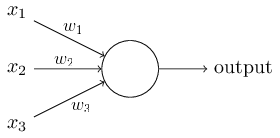
\includegraphics[height=1in, keepaspectratio=true]{perceptron_n.png}
\caption{Perceptron}
\end{figure}\\
Biểu diễn đại số:
\[
  output = 
  \bigg\{
    _{0 \quad if \, \sum_j w_j x_j \, \leq \, threshold}
    ^{1 \quad if \, \sum_j w_j x_j \, > \, threshold}
\]
Các hàm số như trên được gọi là hàm hoạt động - activation function, có nhiều 
loại hàm hoạt động khác nhau như: $sigmoid , tang ...$
\subsubsection{MNN (Multilayer Neural Network)}
MNN được cấu thành bằng cách sắp xếp các perceptron thành 
từng lớp. Các perceptron ở mỗi lớp sẽ kết nối với tất cả các perceptron ở các 
lớp liền kề, lớp những perceptron đầu tiên được gọi là lớp đầu vào (input layer), 
chúng có chức năng tiếp nhận các giá trị đầu vào để cung cấp cho các lớp tiếp 
theo. Các giá trị đầu ra ở lớp trước sẽ chính là các giá trị đầu vào cho 
các perceptron ở lớp tiếp theo. Các perceptron ở lớp cuối cùng được gọi là lớp 
đầu ra (output layer), trong trường hợp này đặc biệt chỉ có duy nhất một 
perceptron ở lớp đầu ra. Còn lại các lớp perceptron khác được gọi là lớp ẩn 
(hidden layer).\\
\begin{figure}[h!]
\centering
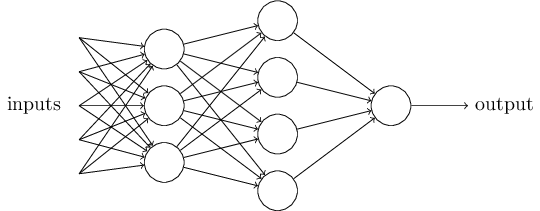
\includegraphics[height=1.25in, keepaspectratio=true]{multilayerneuralnetwork.png}
\caption{MNN}
\end{figure}\\
Giả sử đầu vào của perceptron là $x_1, x_2, ...$ tương ứng là đó là các trọng 
số $w_1, w_2, ...$. Thêm vào định nghĩa về $bias$, ở đây $bias$ là một giá trị 
đại diện độ lệch của từng perceptron và được ký hiệu $b_1, b_2, ...$. Ta có 
biểu diễn của hàm hoạt động với $bias$:
\[
  output = 
  \bigg\{
    _{0 \quad if \, \sum_j w_j x_j + b_i\, \leq \, 0}
    ^{1 \quad if \, \sum_j w_j x_j + b_i\, > \, 0}
\]
\subsubsection{Hàm sigmoid}
Với hàm hoạt động được định nghĩa như trên, giá trị của hàm hoạt động trên lý 
thuyết là không có giới hạn, nghĩa là $output\in\mathbb{R}$. Trong một trường 
hợp cụ thể, với việc sử dụng hàm hoạt động như trên có thể dẫn đến trường hợp 
đầu ra của một perceptron sẽ nhận giá trị rất lớn - giả sử là 1000, những một 
perceptron khác sẽ nhận giá trị rất bé - giả sử 0.001. Vì thế khi đến lớp tiếp 
theo thì gần như perceptron cho kết quả đầu ra là giá trị bé sẽ mất đi độ ảnh 
hưởng và làm mất cân đối cho toàn mạng.\\\\
Do đó để giới hạn giá trị đầu ra của hàm hoạt động chúng ta sẽ sử dụng hàm 
sigmoid. Hàm sigmoid được định nghĩa như sau:
\[
  \sigma(z)=\frac{1}{1+e^{-z}}
\]
Với biễu diễn đồ thị:
\begin{figure}[h!]
\centering
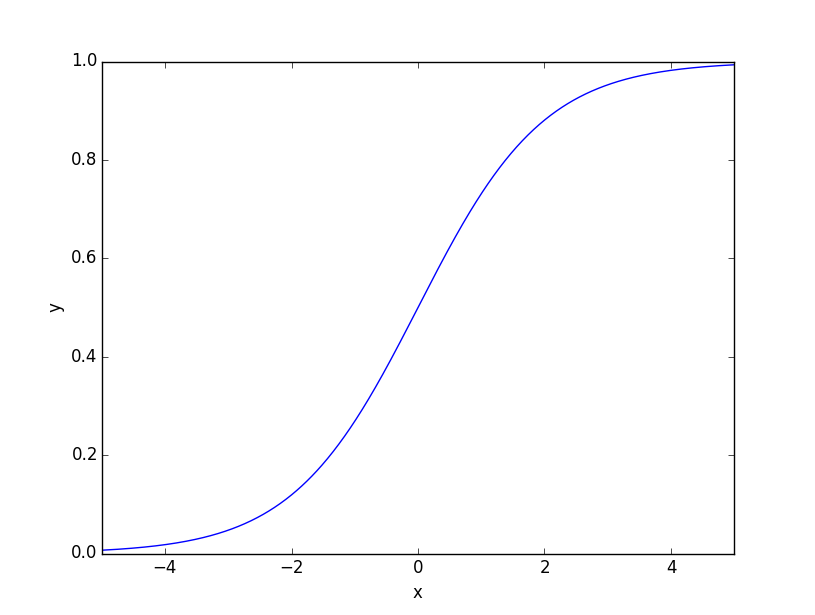
\includegraphics[height=2in, keepaspectratio=true]{sigmoid.png}
\caption{Đồ thị hàm sigmoid}
\end{figure}\\
Áp dụng hàm sigmoid vào hàm hoạt động ta có một hàm hoạt động dạng sigmoid và 
khi đó hàm hoạt động của chúng ta của chúng ta sẽ có dạng:
\[
  \frac{1}{1+exp(-\sum_j w_j x_j -b)}
\]
Lúc này ta có một hàm hoạt động có giá trị được giới hạn trong khoảng từ 0 đến 
1. Nhưng chú ý, giá trị đầu ra của hàm hoạt động vẫn là giá trị liên tục, để 
rời rạc hóa giá trị đầu ra của hàm hoạt động ta có thể sử dụng một phương pháp 
quen thuộc - sử dụng ngưỡng. Điển hình ta chọn ngưỡng $threshold = 0.5$, nếu 
lớn hơn ngưỡng thì giá trị đầu ra của hàm hoạt động sẽ nhận 1 và ngược lại sẽ 
nhận 0.
\subsubsection{Giải thuật lan truyền ngược}
Giải thuật lan truyền ngược cung cấp cho mạng neural khả năng tự học hỏi từ 
đó để bản thân mạng có thể tự xây dựng mô hình 
quyết định và đưa ra các giá trị đầu ra tương ứng với từng trường hợp đầu vào 
cụ thể.\\\\
Cụ thể, MNN với hàm hoạt động có dạng
sigmoid và các tham số $w, b$, các tham số này chưa có giá trị.  Việc cung 
cấp khả năng tự học hỏi cho mạng chính là cung cấp một giải thuật giúp mạng 
tìm được các tham số $w, b$ với một tập kinh nghiệm - hay tập huấn luyện - 
${x, y}$ cụ thể, trong đó $x$ là giá trị đầu vào và $y$ là giá trị đầu ra 
tương ứng với từng bộ $x$. Giải thuật lan truyền ngược là một giải thuật giúp 
giải quyết vấn đề trên.\\\\
Biểu diễn trọng số, $bias$ và hàm hoạt động:\\\\
Trọng số $w_{jk}^\ell$ là trọng số từ lớp perceptron thứ $k$ của lớp $(\ell-1)$ 
đến perceptron thứ j thuộc lớp thứ $\ell$.
Như hình trên, trọng số xuất phát từ perceptron thứ 4 thuộc lớp thứ 2 và kết 
thúc tại perceptron thứ 2 thuộc lớp thứ 3 được ký hiệu là $w_{24}^3$.\\
\begin{figure}[h!]
\centering
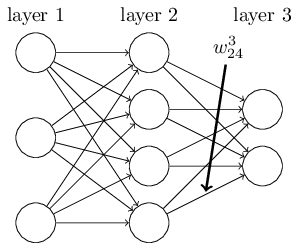
\includegraphics[height=2in, keepaspectratio=true]{exw.png}
\caption{Ký hiệu trọng số}
\end{figure}\\
Tương tự như vậy với $bias$ và hàm hoạt động của perceptron thứ $j$ thuộc lớp 
thứ $\ell$ của mạng sẽ được kí hiệu thứ tự là $b_j^\ell,\,a_j^\ell$. Ví dụ, $bias$ 
của perceptron thứ 3 thuộc lớp thứ 2 sẽ là $b_3^2$ và hàm hoạt động của 
perceptron thứ 1 thuộc lớp thứ 3 sẽ là $a_1^3$.\\
\begin{figure}[h!]
\centering
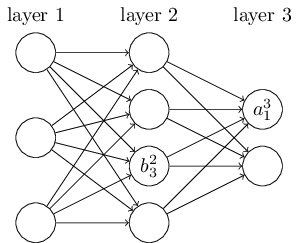
\includegraphics[height=2in, keepaspectratio=true]{exb.png}
\caption{Ký hiệu $bias$}
\end{figure}\\
Biễu diễn ma trận trọng số và vector $bias$:
\begin{itemize}
\item $w$ là ma trận của các giá trị trọng số.
\[ w =
\begin{bmatrix}
w_{11} & \ldots & w_{1k} \\
\vdots & \ddots & \vdots\\
w_{j1} & \ldots & w_{jk}
\end{bmatrix}
\]
\item $b$ là vector của các giá trị $bias$.
\[ b =
\begin{bmatrix}
b_1\\
\vdots\\
b_k
\end{bmatrix}
\]
\item $\sigma$ là hàm sigmoid.
\item $a_j=\sigma$ là hàm hoạt động có dạng sigmoid, $a$ là vector của các hàm 
hoạt động.
\[ a =
\begin{bmatrix}
a_1\\
\vdots\\
a_k
\end{bmatrix}
\]
\end{itemize}
Lúc này ta có biểu diễn toán học đầy đủ của hàm hoạt động:
\[
  a_j^\ell=\sigma(\sum_k w_{jk}^\ell a_k^{\ell-1} + b_j^\ell)=\sigma(z _j^\ell)
\]
\[
  z _j^\ell=\sum_k w_{jk}^\ell a_k^{\ell-1} + b_j^\ell
\]
Tổng quát phát biểu với dạng:\\
\[
  a^\ell=\sigma(w^\ell a^{\ell-1} + b^\ell)=\sigma(z^\ell)
\]
Để có thể tìm được giá trị của các biến $w$ và $b$, giải thuật lan truyền ngược 
thực hiện bằng cách xuất phát $w$ và $b$ từ các giá trị ngẫu nhiên, thực hiện 
các phép lặp để đưa $w$ và $b$ về giá trị đúng, mỗi lần lặp sẽ có một hàm chi 
phí (cost function) đo đạc độ lệch của giá trị tính toán và giá trị thực tế 
để giúp giải thuật tìm được giá trị hội tụ.\\\\
Biễu diễn hàm chi phí với $L$ lớp:
\[
  C=\frac{1}{2n}\sum_x\|y(x)-a^L(x)\|^2
\]
Ta có thể thấy, dạng hàm số trên tương đồng với định nghĩa độ lệch chuẩn trong 
xác suất thống kê nhưng có một số biến đổi khác biệt. Thay vì giá trị kỳ vọng 
và các giá trị xác suất, hàm chi phí sử dụng giá trị thực tế $y$ của tập dữ 
liệu và giá trị $y=a$ là giá trị $y$ tính toán được từ $x$ với $w$ và $b$. Vậy 
ta có thể hiểu được, hàm chi phí tính toán độ sai lệch của giá trị $a$ so với 
$y$ kỳ vọng thực tế. Do đó, hàm chi phí càng nhỏ thì biểu diễn giá trị của 
MNN sẽ càng gần với thực tế.\\\\
Để tìm được giá trị cực tiểu cho hàm chi phí ta sẽ thực hiện vòng lặp:
\[
  w_{jk}^\ell:=w_{jk}^\ell-\eta\frac{\partial}{\partial w_{jk}^\ell}C(w,b)
\]
\[
  b_j^\ell:=b_j^\ell-\eta\frac{\partial}{\partial b_j^\ell}C(w,b)
\]
Trong đó $\eta$ là tỉ lệ học (learning rate), việc hội tụ về giá trị cực tiểu 
với tốc độ và độ chính xác phụ thuộc vào tỉ lệ này. Thực hiện được hai vòng lặp 
trên, ta sử dụng giải thuật lan truyền ngược để tính toán 
$\frac{\partial}{\partial w_{jk}^\ell}C(w,b)$ và 
$\frac{\partial}{\partial b_j^\ell}C(w,b)$.\\\\
Tham số lỗi $\delta_j^\ell$ của neural thứ $j$ thuộc lớp $\ell$ là biểu diễn 
của:
\[
  \delta_j^\ell \equiv \frac{\partial C}{\partial z_j^\ell}
\]
Từ biểu diễn trên ta có:
\[
  \delta_j^L = \frac{\partial C}{\partial a_j^L} \sigma'(z_j^L)
\]
Mặc khác $\partial C/\partial a_j^L = (a_j^L-y_j)$, suy ra:
\[
  \delta^L=\nabla_aC\odot\sigma'(z^L)=(a^L-y)\odot\sigma'(z^L)
\]
Trong đó $\odot$ là tích Hadamard, ta gọi biểu thức trên là biểu thức (3.1).
Ngoài ra, ta có biểu diễn khác của $\delta_j^L$:
\begin{align*}
  \delta_j^L=\frac{\partial C}{\partial z_j^L}
  &=\sum_k\frac{\partial C}{\partial z_k^{\ell+1}}\frac{\partial z_k^{\ell+1}}{\partial z_j^\ell}\\
  &=\sum_k\frac{\partial z_k^{\ell+1}}{\partial z_j^\ell}\delta_k^{\ell+1}\\
  &=\sum_k\frac{\partial(\sum_j w_{kj}^{\ell+1}a_j^\ell+b_k^{\ell+1})}{\partial z_j^\ell}\delta_k^{\ell+1}\\
  &=\sum_k\frac{\partial(\sum_j w_{kj}^{\ell+1}\sigma(z_j^\ell)+b_k^{\ell+1})}{\partial z_j^\ell}\delta_k^{\ell+1}\\
  &=\sum_k w_{kj}^{\ell+1}\delta_k^{\ell+1}\sigma'(z_j^\ell)
\end{align*}
Gọi biểu thức trên là biểu thức (3.2). Với hướng tiếp cận tương tự ta có các 
biểu thức khác:
\begin{align*}
  \frac{\partial C}{\partial b_j^\ell}&=\frac{\partial C}{\partial z_j^\ell}\frac{\partial z_j^\ell}{\partial b_j^\ell}\\
  &=\delta_j^\ell\frac{\partial z_j^\ell}{\partial b_j^\ell}\\
  &=\delta_j^\ell\frac{\partial(\sum_k w_{jk}^\ell a_k^{\ell-1} + b_j^\ell)}{\partial b_j^\ell}\\
  &=\delta_j^\ell
\end{align*}
Ta có biểu thức trên là biểu thức (3.3).
\begin{align*}
  \frac{\partial C}{\partial w_{jk}^\ell}&=\frac{\partial C}{\partial z_j^\ell}\frac{\partial z_j^\ell}{\partial w_{jk}^\ell}\\
  &=\delta_j^\ell\frac{\partial(\sum_k w_{jk}^\ell a_k^{\ell-1} + b_j^\ell)}{\partial w_{jk}^\ell}\\
  &=\delta_j^\ell a_k^{\ell-1}
\end{align*}
Và biểu thức (3.4). Từ (3.1), (3.2), (3.3) và (3.4) ta có tổng kết sau:
\begin{align}
  \delta^L =& \: \nabla_aC\odot\sigma'(z^L) \\
  \delta^\ell =& \: ((w^{\ell+1})^T\delta^{\ell+1})\odot\sigma'(z^\ell) \\
  \frac{\partial C}{\partial b_j^\ell} =& \: \delta_j^\ell \\
  \frac{\partial C}{\partial w_{jk}^\ell} =& \: a_k^{\ell-1}\delta_j^\ell
\end{align}
Sử dụng các biểu thức này, giải thuật lan truyền ngược dùng để tính toán 
$\frac{\partial}{\partial w_{jk}^\ell}C(w,b)$ và 
$\frac{\partial}{\partial b_j^\ell}C(w,b)$ được mô tả các bước như sau:
\begin{enumerate}
\item Cho giá trị đầu vào $x$, tính toán giá trị $a^1$ tương ứng với $x$.
\item Với mỗi $\ell=2,3,..,L$, ta lần lượt tính được $z^\ell=w^\ell a^{\ell-1}+b^\ell$ 
và $a^\ell=\sigma(z^\ell)$.
\item Tính giá trị của vector $\delta^L=\nabla_aC\odot\sigma'(z^L)$.
\item Từ giá trị của $\delta^L$ ta có thể tính được giá trị của các tham số lỗi 
còn lại, với mỗi $\ell=L-1,L-2,...,2$ ta thực hiện $\delta^\ell=((w^{\ell+1})^T\delta^{\ell+1})\odot\sigma'(z^\ell)$.
\item Kết thúc quá trình tính toán với $\frac{\partial C}{\partial w_{jk}^\ell}=a_k^{\ell-1}\delta_j^\ell$ và 
$\frac{\partial C}{\partial b_j^\ell}=\delta_j^\ell$.
\end{enumerate}
\subsubsection{Thông số đánh giá}
Có ba tham số cơ bản dùng để xem xét và đánh giá kết quả giải thuật trong Học máy.
Ký hiệu: \textbf{True positive} là $TP$, \textbf{False positive} là $FP$, 
\textbf{True negative} là $TN$, \textbf{False negative} là $FN$.\\\\
Ta có:
\[
  Accuracy = \frac{TP+TN}{TP+FP+TN+FN}
\]
\[
  Precision = \frac{TP}{TP+FP}
\]
\[
  Recall = \frac{TP}{TP+FN}
\]
\begin{figure}[h!]
\centering
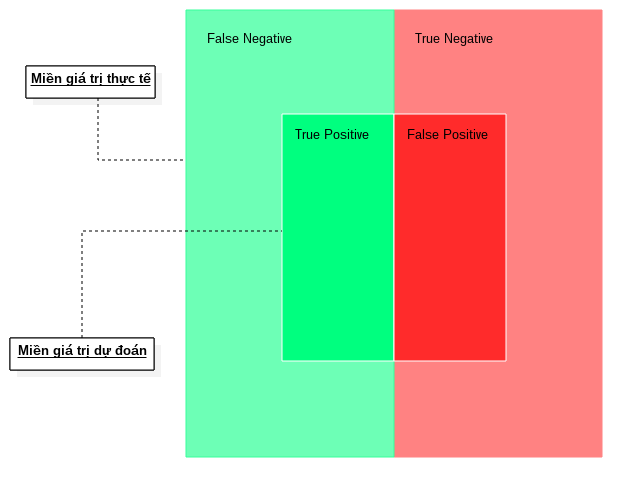
\includegraphics[height=2.5in, keepaspectratio=true]{precision_recall.png}
\caption{Thông số đánh giá}
\end{figure}